\begin{figure}
\centering
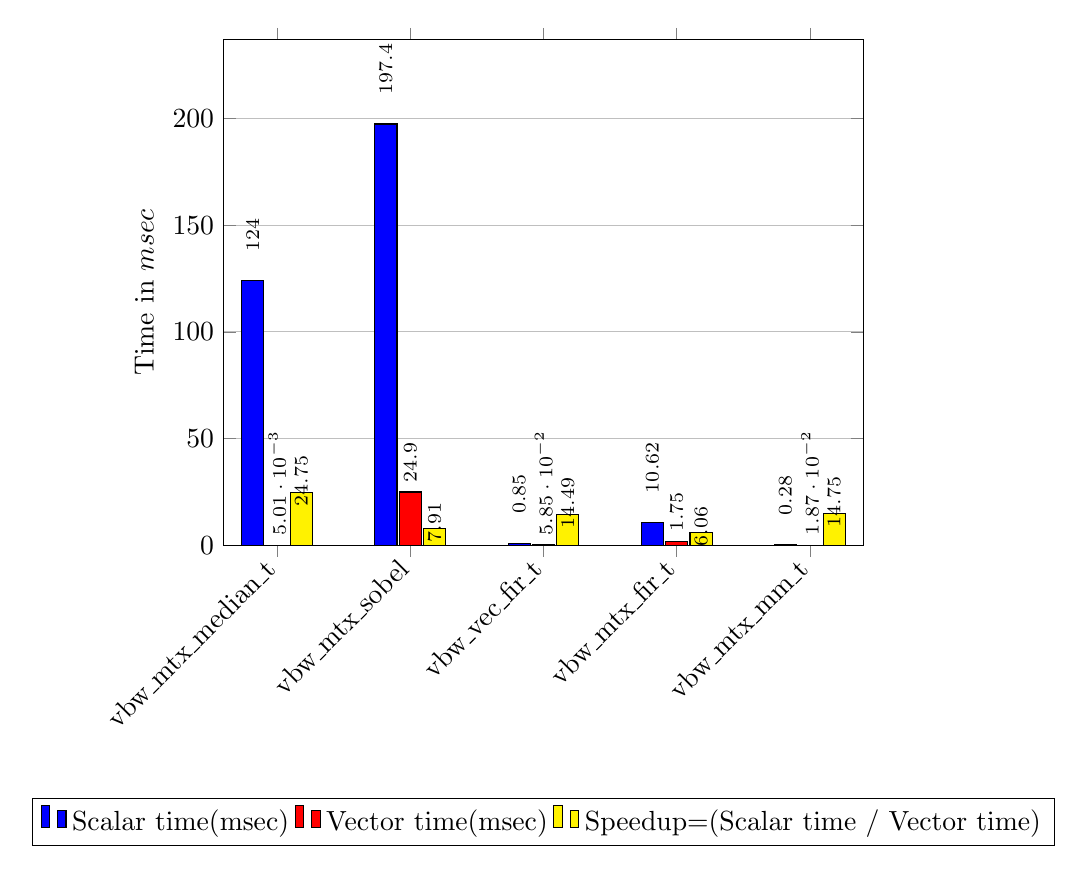
\begin{tikzpicture}
\begin{axis}[
width  = 0.8*\textwidth,
height = 8cm,
%major x tick style = transparent,
x tick label style={rotate=45, anchor=east, align=right,text width=4cm},
bar width=8pt,
ymajorgrids = true,
ylabel = {Time in $msec$},
symbolic x coords={vbw\_mtx\_median\_t,vbw\_mtx\_sobel,vbw\_vec\_fir\_t,vbw\_mtx\_fir\_t,vbw\_mtx\_mm\_t},
xtick = data,
nodes near coords,
ybar,
every node near coord/.append style={rotate=90, anchor=west, font=\scriptsize, xshift=0.25cm},
scaled y ticks = false,
enlarge y limits={upper,value=0.2},
%enlarge x limits=0.25,
ybar=2*\pgflinewidth,
legend cell align=left,
legend style={
	at={(.5,-0.5)},
	anchor=north,
	legend columns=-1
	column sep=0.5ex
}
]
\addplot[draw=black,fill=blue]
coordinates {(vbw\_mtx\_median\_t, 124) (vbw\_mtx\_sobel,197.4) (vbw\_vec\_fir\_t,0.847) (vbw\_mtx\_fir\_t,10.62) (vbw\_mtx\_mm\_t,0.276)};

\addplot[draw=black,fill=red, every node near coord/.append style={xshift=-0.25cm}]
coordinates {(vbw\_mtx\_median\_t, 0.005012) (vbw\_mtx\_sobel,24.9) (vbw\_vec\_fir\_t,0.0585) (vbw\_mtx\_fir\_t,1.75) (vbw\_mtx\_mm\_t,0.01865)};

\addplot[draw=black,fill=yellow,every node near coord/.append style={xshift=-0.55cm}]
coordinates {(vbw\_mtx\_median\_t,24.75) (vbw\_mtx\_sobel,7.911) (vbw\_vec\_fir\_t,14.49) (vbw\_mtx\_fir\_t,6.057) (vbw\_mtx\_mm\_t,14.75)};

%nodes near coords=\raisebox{1.7cm}{\pgfmathprintnumber\pgfplotspointmeta}

\legend{Scalar time(msec),Vector time(msec), Speedup=(Scalar time / Vector time)}
\end{axis}
\end{tikzpicture}
\caption{Speedup for different benchmarks}
\label{g1:g1}
\end{figure}